\documentclass{beamer}

\usepackage{braket}
\usepackage{multirow}
\usepackage{feynmp-auto}
\usepackage{amsmath}
\usepackage{amssymb}
\usepackage{graphicx}
\usepackage{dsfont}

\mode<presentation> {\usetheme{Madrid}}
\usepackage{graphicx} 
\usepackage{booktabs} 

\title[Nuclear Momentum Distributions]{Nuclear Momentum Distributions} 

\author{Jarrick Nys}
\institute[UGent] {Universiteit Gent}
\date{28/01/2015} 

\begin{document}

\begin{frame}
\titlepage 
\end{frame}

\begin{frame}
\frametitle{Overview} 
\tableofcontents 
\end{frame}
\section{One body momentum distribution}
\begin{frame}
\frametitle{One body momentum distribution}
Chance of finding a particle with momentum $[k,k+dk]$ is $n_1(k) k^2dk$
\begin{equation*} \label{eq:one_patricle_distr}
	n_1(\vec{k})=\frac{1}{(2\pi)^3}\int d\vec{r}_1 \int d\vec{r}_1^{\ \prime} e^{i\vec{k}\cdot (\vec{r}_1-\vec{r}^{\ \prime}_1)}\rho_1(\vec{r}_1,\vec{r}_1^{\ \prime}).
\end{equation*}
$\rho_1(\vec{r}_1,\vec{r}_1^{\ \prime})$ is the one-body non-diagonal density matrix
\begin{equation*}
\rho_1(\vec{r}_1,\vec{r}^{\ \prime}_1) = \int \{d\vec{r}_{2-A}\} \Psi^*_A(\vec{r}_1,\vec{r}_2,\vec{r}_3, ... ,\vec{r}_A)\Psi_A(\vec{r}_1^{\ \prime},\vec{r}_2,\vec{r}_3, ... ,\vec{r}_A).
\end{equation*}
\end{frame}

\begin{frame}
\frametitle{One body momentum distribution}
In the second quantization formalism
\begin{equation*}
n_1(\vec{k})= \frac{1}{A}\bra{\Psi_A} \psi^\dagger(\vec{k}) \psi(\vec{k})\ket{\Psi_A}
\end{equation*}
and
\begin{equation*}
\rho_1(\vec{r}_1,\vec{r}^{\ \prime}_1)= \frac{1}{A}\bra{\Psi_A} \psi^\dagger(\vec{r}_1) \psi(\vec{r}^{\ \prime}_1)\ket{\Psi_A}
\end{equation*}

\begin{figure}
\centering
\begin{fmffile}{dianpd}
\large % change font size
\boldmath % math in bold
\begin{fmfgraph*}(80,50)
\fmfstraight
\fmfleft{i1,i2,i3,i4,i5,i6}
\fmfright{o1,o2,o3,o4,o5,o6}
\fmf{plain}{i1,v1,o1}
\fmf{plain}{i2,v2,o2}
\fmf{plain}{i3,v3,o3}
\fmf{plain,tension=0.4}{i4,v4}
\fmf{plain,tension=0.4}{v5,o4}
\fmf{fermion,label=$\vec{k}$,label.side=left}{v4,v6}
\fmf{fermion,label=$\vec{k}$, label.side=left}{v7,v5}
\fmfdot{v4,v5}
\fmfforce{(0.3w,1.0h)}{v6}
\fmfforce{(0.7w,1.0h)}{v7}
\fmfforce{(0.3w,0.6h)}{v4}
\fmfforce{(0.7w,0.6h)}{v5}
\end{fmfgraph*}
\end{fmffile}
\end{figure}
\end{frame}

\section{OBMD for Independent Particle Model}

\begin{frame}
\frametitle{OBMD for Independent Particle Model}
Particles move independent in potential $\rightarrow$ Nuclear wave function = Slater determinant of one-particle wave functions
\begin{equation*} \label{eq:slater}
\Psi_A(\vec{r}_1,\vec{r}_2,\vec{r}_3, ... ,\vec{r}_A)= \frac{1}{\sqrt{A!}} \sum_{\substack{i_1 i_2 \ldots i_A}} 
													  \varepsilon_{i_1 i_2 \ldots i_A}\  \phi_{i_1}(\vec{r}_1)
													         \phi_{i_2}(\vec{r}_2)...
													         \phi_{i_A}(\vec{r}_A).
\end{equation*}
One obtains for the one-body momentum distribution 
\begin{align*} 
	n_1(\vec{k})= \frac{1}{A} \sum_{\substack{i}} \tilde{\phi}^*_i(\vec{k})\tilde{\phi}_i(\vec{k}).
\end{align*}

\end{frame}

\section{OBDM for Spherical Harmonic Oscillator potential}

\begin{frame}
\frametitle{OBDM for Spherical Harmonic Oscillator potential}
Time independent Schrodinger equation for the nucleons
\begin{equation*} \label{eq:HO}
\left( -\frac{\hbar^2}{2M_N} \nabla^2 + \frac{1}{2} M_N \omega^2 r^2 \right) \phi_{nlm}(\vec{r}) = E\phi_{nlm}(\vec{r}).
\end{equation*}
with solutions 
\begin{equation*}
 \phi_{nlm}(\vec{r}) = \left[ \frac{2n!}{\Gamma(n+l+\frac{3}{2})}\nu^{l+\frac{3}{2}} \right]^{\frac{1}{2}} r^l e^{-\frac{\nu r^2}{2}} L^{l+\frac{1}{2}}_n(\nu r^2) \times Y_{lm}(\Omega) 
\end{equation*}
with
\begin{equation*}
\nu \equiv \frac{M_N \omega}{\hbar}.
\end{equation*}
The parameter $\hbar\omega$ can be parameterized
\begin{equation*}
\hbar\omega (MeV) = 45A^{-1/3}-25A^{-2/3}
\end{equation*}
\end{frame}

\begin{frame}
\frametitle{OBDM for Spherical Harmonic Oscillator potential}
In momentum space Schrodinger equation has same form, so solutions have same form
\begin{align*}
 \tilde{\phi}_{nlm}(\vec{k}) & = K_{nl}(k)Y_{lm}(\Omega_k) \\
 & = \left[ \frac{2n!}{\Gamma(n+l+\frac{3}{2})}\nu'^{l+\frac{3}{2}} \right]^{\frac{1}{2}} k^l e^{-\frac{\nu' k^2}{2}} L^{l+\frac{1}{2}}_n(\nu' k^2) \times Y_{lm}(\Omega_k)
\end{align*}
with
\begin{equation*}
\nu^{\prime} \equiv \frac{\hbar}{M_N \omega}.
\end{equation*}
$L^\alpha_n$  : generalized Laguerre polynomals\\
$Y_{lm}$ : Spherical harmonics

\end{frame}

\begin{frame}
One can now calculate the one-body momentum distribution
\begin{equation*}
\tilde{\phi}_{nlm}(\vec{k}) \equiv \braket{\vec{k}|nlm} = K_{nl}(k)Y_{lm}(\Omega_k)	
\end{equation*}
\begin{align*}
n_1(k) & = \frac{2}{A} \sum_{nlm} K^2_{nl}(k) \int d\Omega_k Y^*_{lm}(\Omega_k)  Y_{lm}(\Omega_k) \\
& =  \frac{2}{A} \sum_{nl} (2l+1) K^2_{nl}(k) .
\end{align*}
The sum goes over all $n,l$ of the occupied states. 
\end{frame}

\section{Results}
\begin{frame}
\frametitle{Results}
Norm = 1
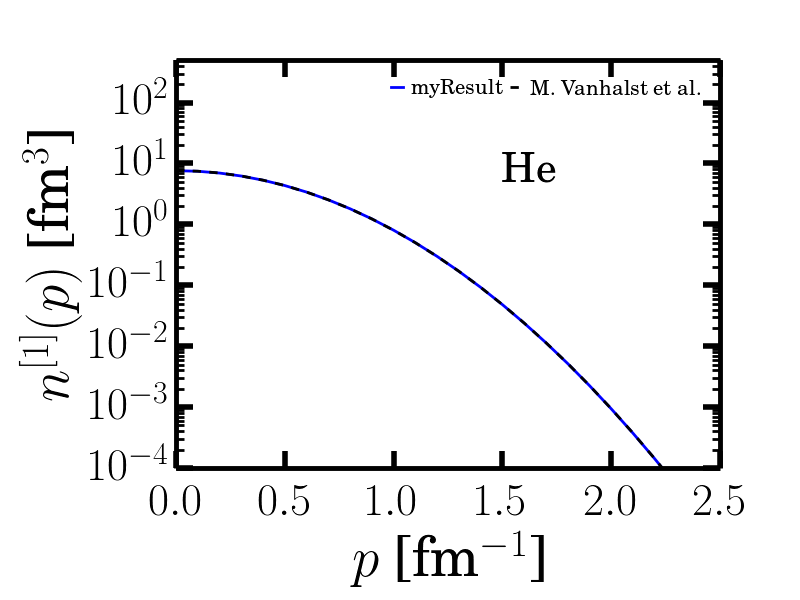
\includegraphics[scale=0.5]{He_mf.png} 
\end{frame}

\begin{frame}
\frametitle{Results}
Norm = 1
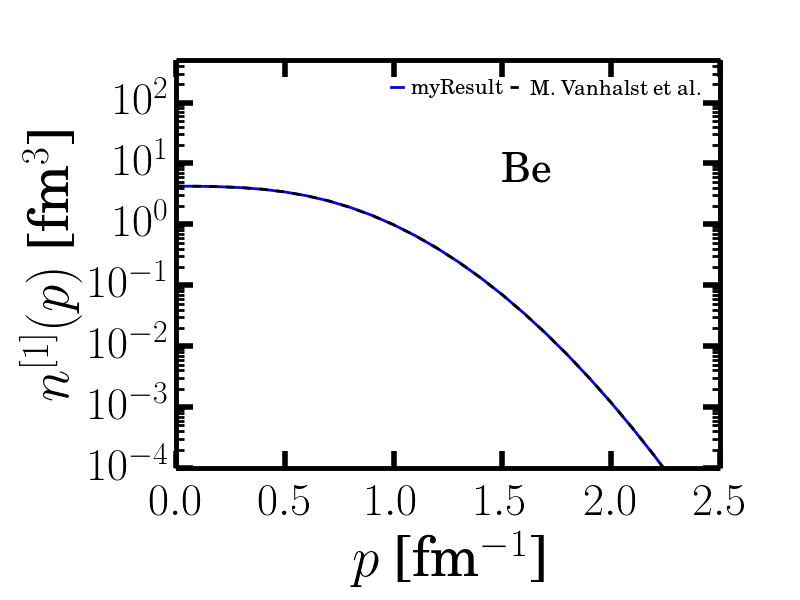
\includegraphics[scale=0.5]{Be_mf.png} 
\end{frame}
\begin{frame}
\frametitle{Results}
Norm = 1
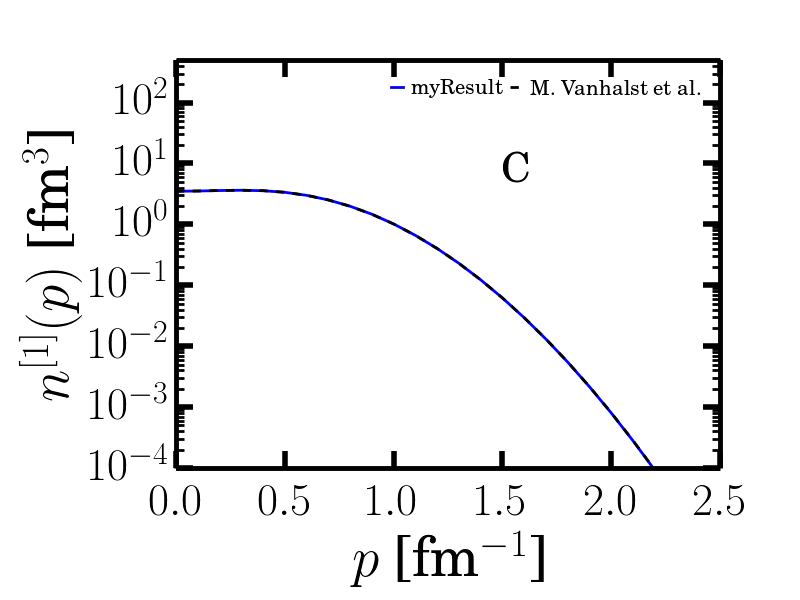
\includegraphics[scale=0.5]{C_mf.png} 
\end{frame}
\begin{frame}
\frametitle{Results}
Norm = 1
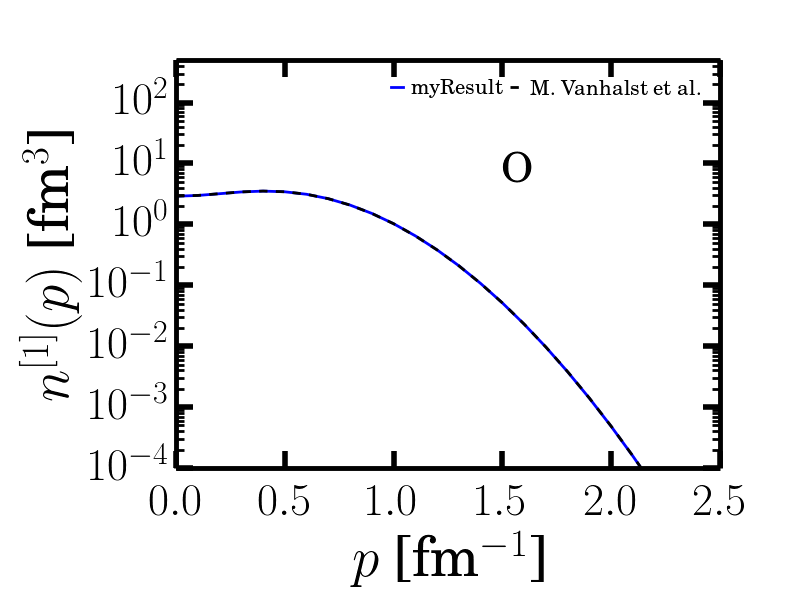
\includegraphics[scale=0.5]{O_mf.png} 
\end{frame}
\begin{frame}
\frametitle{Results}
Norm = 1
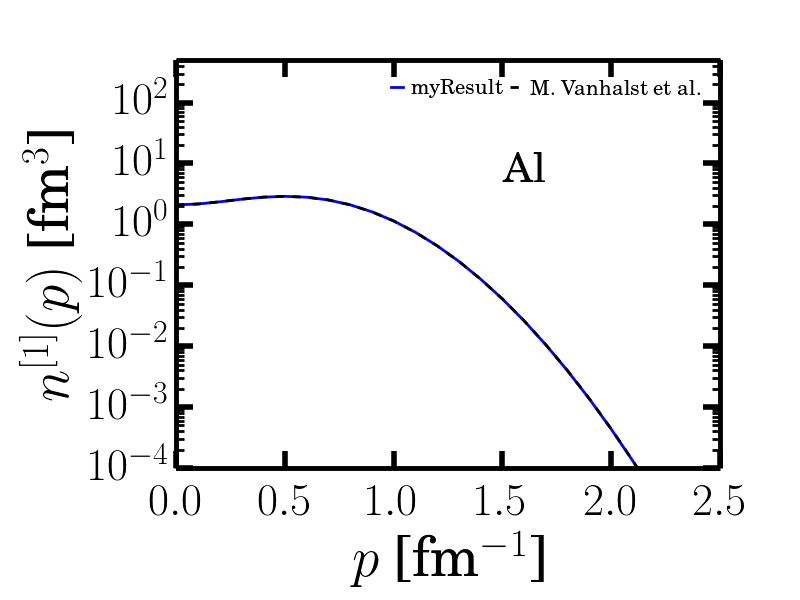
\includegraphics[scale=0.5]{Al_mf.png} 
\end{frame}
\begin{frame}
\frametitle{Results}
Norm = 1
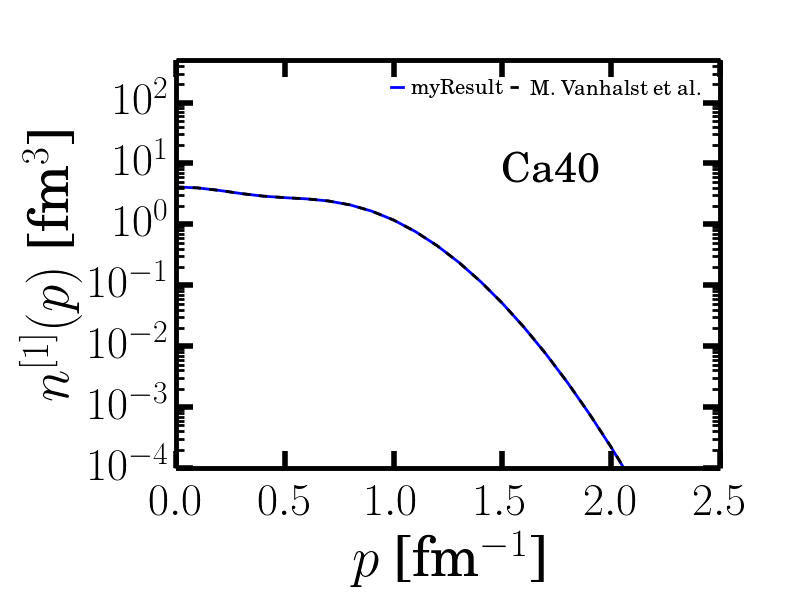
\includegraphics[scale=0.5]{Ca40_mf.png} 
\end{frame}
\begin{frame}
\frametitle{Results}
Norm = 1
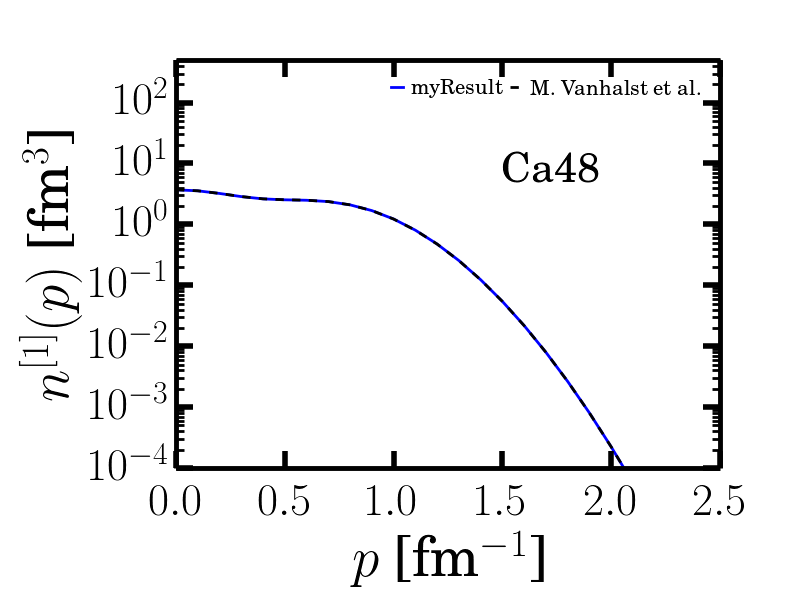
\includegraphics[scale=0.5]{Ca48_mf.png} 
\end{frame}
\begin{frame}
\frametitle{Results}
Norm = 1
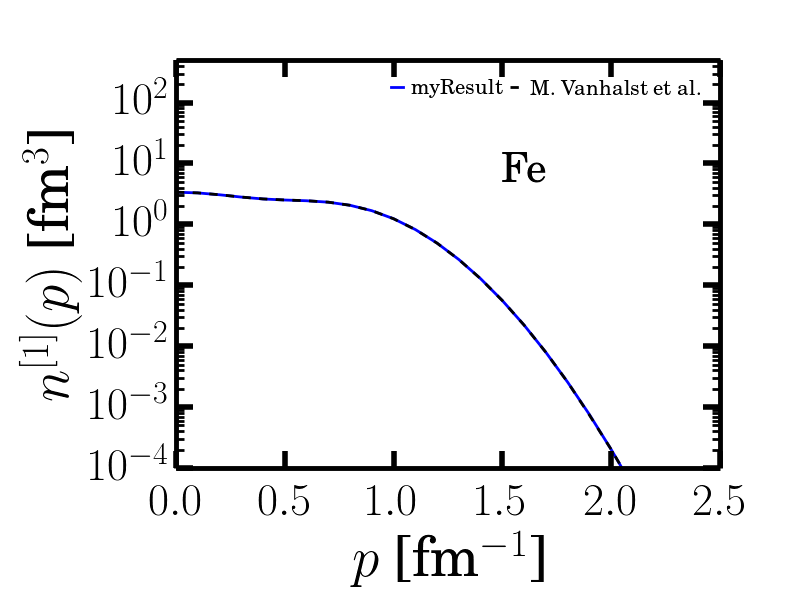
\includegraphics[scale=0.5]{Fe_mf.png} 
\end{frame}
\begin{frame}
\frametitle{Results}
Norm = 1
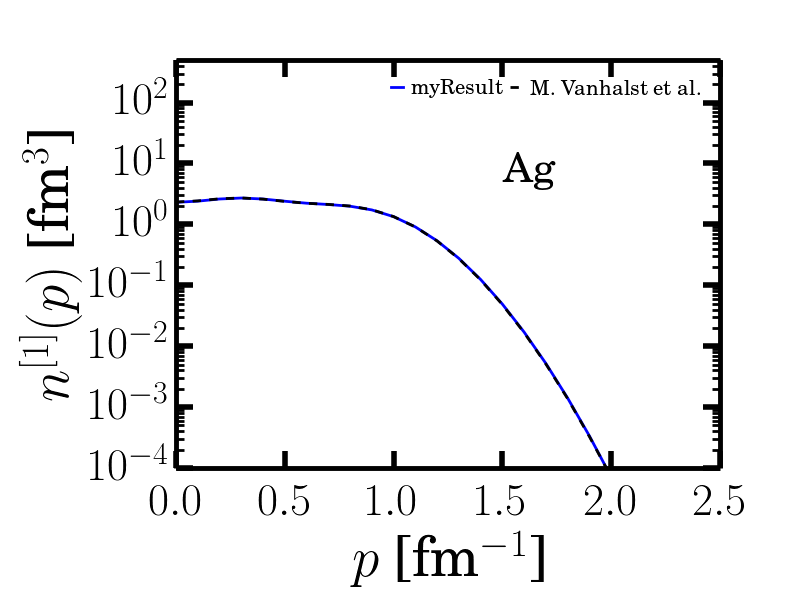
\includegraphics[scale=0.5]{Ag_mf.png} 
\end{frame}

\begin{frame}
\frametitle{Results}
Norm = 1
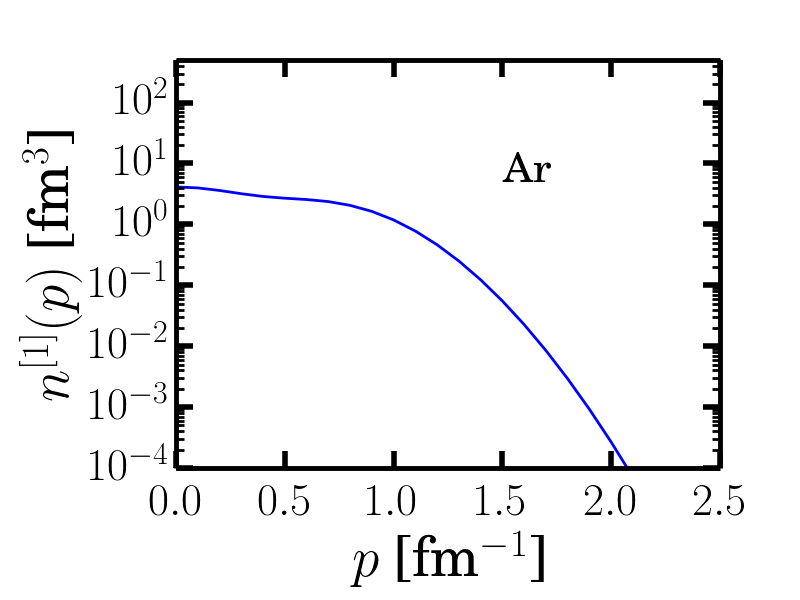
\includegraphics[scale=0.5]{Ar_mymf.png} 
\end{frame}

\begin{frame}
\frametitle{Results}
Norm = 1
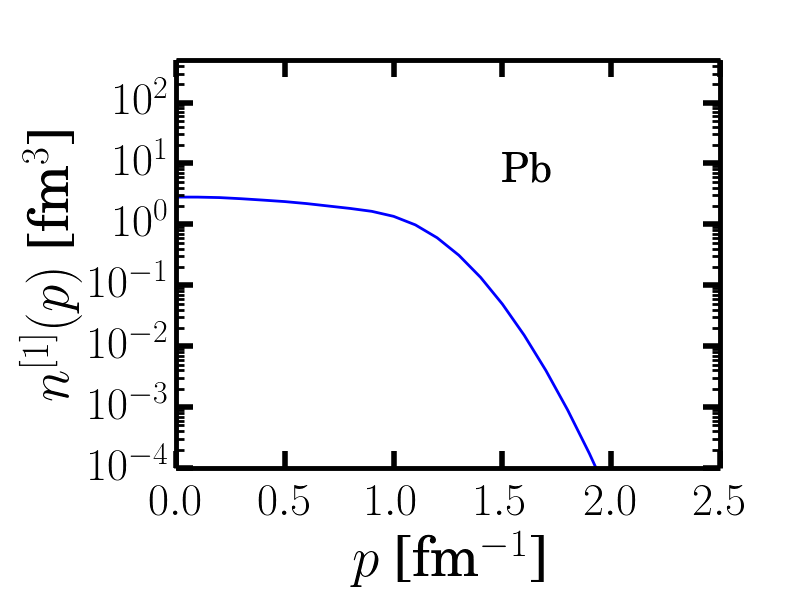
\includegraphics[scale=0.5]{Pb_mymf.png} 
\end{frame}

\begin{frame}
\frametitle{Results}
Normalisation = A
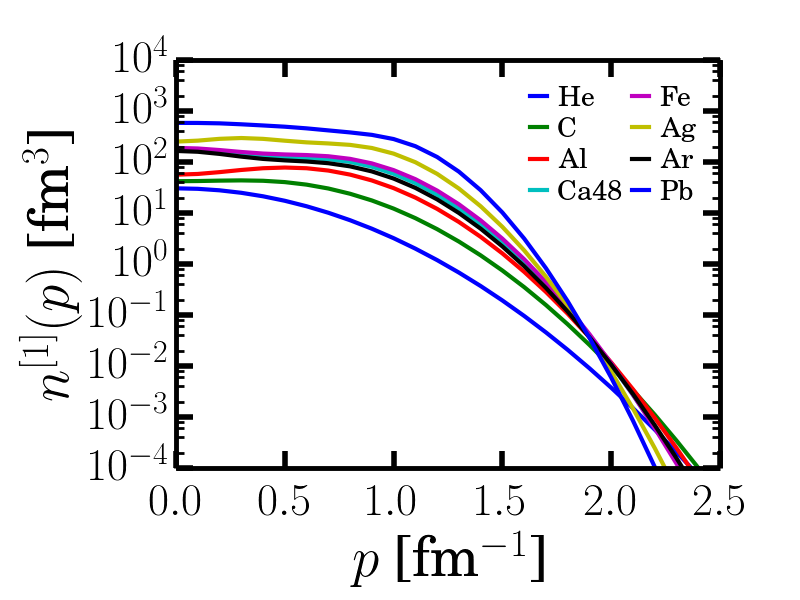
\includegraphics[scale=0.5]{overview.png} 
\end{frame}

\begin{frame}
\frametitle{Results: Discussion}
\begin{itemize}
\item $n_1(k)$ very small for p$\rightarrow \infty$  
\end{itemize}
\end{frame}

\section{Outlook}
\begin{frame}
\frametitle{Outlook}
\begin{itemize}
\item Two-body momentum distribution
\item Try Wood-Saxon potential
\item Introduce correlations
\end{itemize}
\end{frame}

\end{document} 